\chapter{Hasil dan Pembahasan}

\begin{tcolorbox}[title=Daftar Anggota Kelompok]
\begin{enumerate}[noitemsep]
    \item Anggota 1, NIM: 00/000001/PA/00001 --- analisis proses bisnis dan ERD.
    \item Anggota 2, NIM: 00/000002/PA/00002 --- skema relasional dan DDL.
    \item Anggota 3, NIM: 00/000003/PA/00003 --- query 1--3 dan aljabar relasional.
    \item Anggota 4, NIM: 00/000004/PA/00004 --- query 4--5, integrasi, dan validasi.
\end{enumerate}
\textbf{Catatan:} identitas di atas bersifat sementara dan harus diganti sebelum pengumpulan.
\end{tcolorbox}

\section{Entity Relationship Diagram}

Basis data dirancang untuk mempertahankan kronologi kegiatan akademik. Delapan entitas yang digunakan ialah \texttt{program\_studi}, \texttt{mahasiswa}, \texttt{dosen}, \texttt{mata\_kuliah}, \texttt{prasyarat\_mata\_kuliah}, \texttt{semester\_akademik}, \texttt{kelas\_kuliah}, dan \texttt{pengambilan\_kuliah}. Pemisahan data semester, kelas, dan pengambilan membuat setiap riwayat kuliah tersimpan sebagai baris tersendiri sehingga pengulangan mata kuliah tidak menghapus nilai terdahulu.

Satu program studi memiliki banyak mahasiswa dan mata kuliah. Satu mata kuliah dapat ditawarkan dalam banyak kelas pada semester yang berbeda, sedangkan satu kelas hanya mengacu kepada satu mata kuliah, satu semester, dan satu dosen. Dengan demikian, dosen dapat mengajar lebih dari satu kelas paralel, tetapi satu kelas tidak menerapkan \textit{team teaching}. Relasi banyak-ke-banyak antara mahasiswa dan kelas direalisasikan oleh \texttt{pengambilan\_kuliah}.

Prasyarat dimodelkan sebagai relasi rekursif pada \texttt{mata\_kuliah} melalui tabel penghubung \texttt{prasyarat\_mata\_kuliah}. Desain ini memungkinkan satu mata kuliah memiliki beberapa prasyarat dan satu mata kuliah menjadi prasyarat bagi beberapa mata kuliah lain. Atribut \texttt{sifat} membedakan mata kuliah wajib (W) dan pilihan (P).

\begin{figure}[htbp]
    \centering
    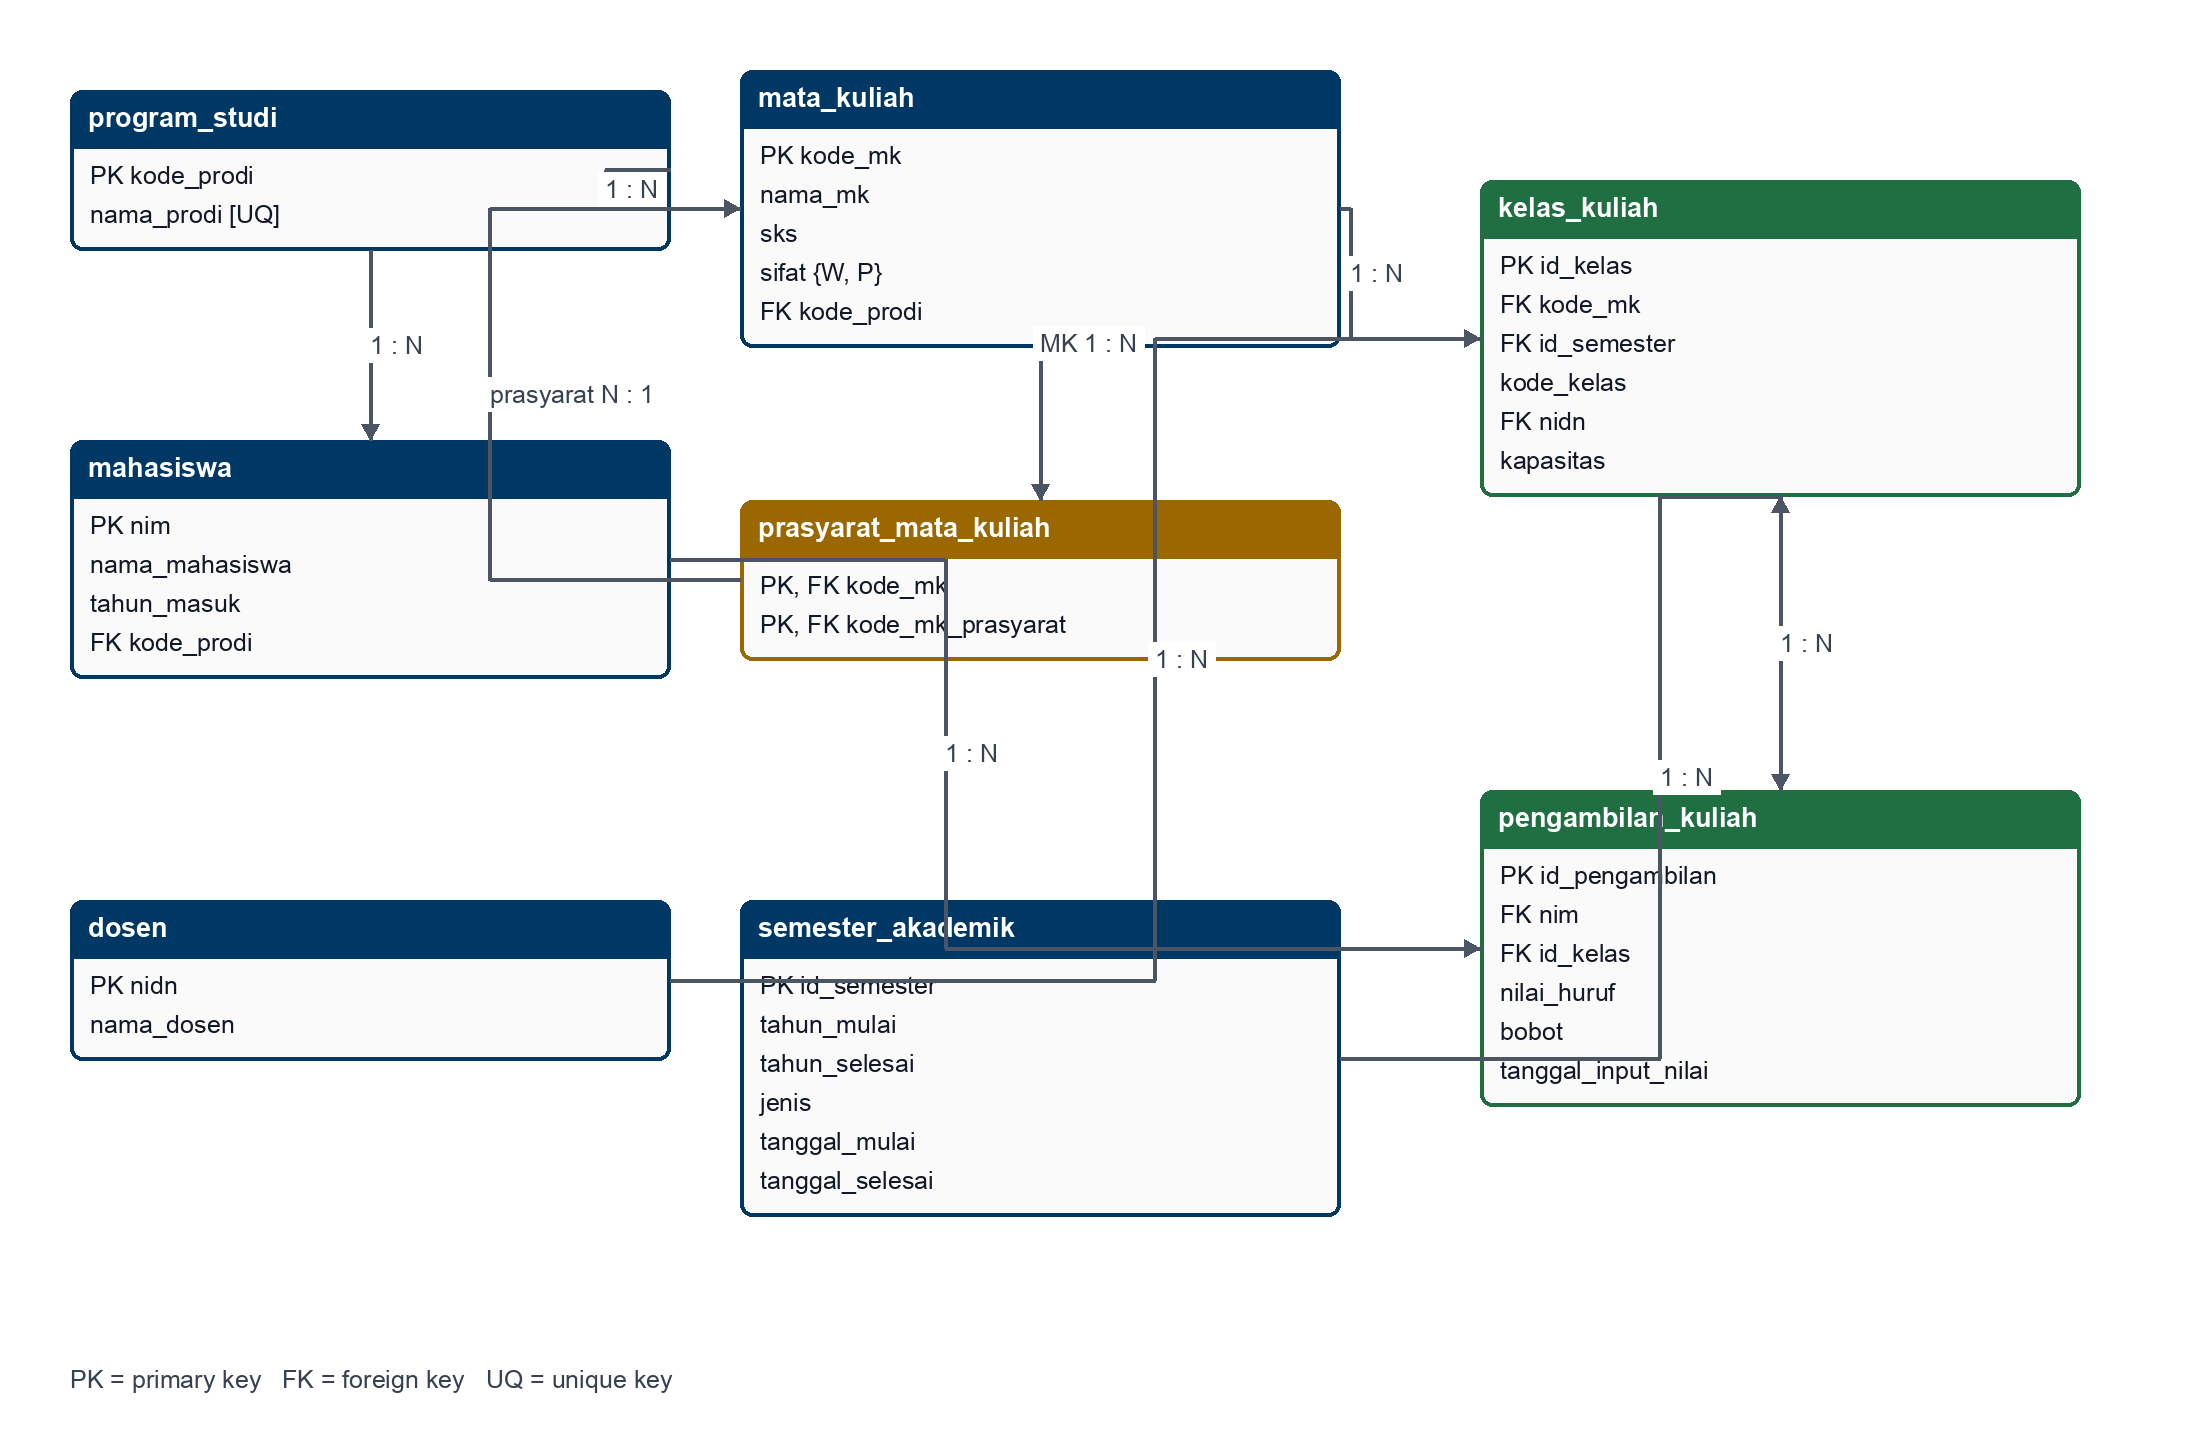
\includegraphics[width=\textwidth]{erd-akademik.png}
    \caption{ERD basis data akademik}
    \label{gb:erd-akademik}
\end{figure}

Nilai mengikuti bobot A=4,00; A-=3,75; A/B=3,50; B+=3,25; B=3,00; B-=2,75; B/C=2,50; C+=2,25; C=2,00; C/D=1,50; D=1,00; dan E=0,00. Angka C/D dan simbol E tersebut digunakan untuk memperbaiki kekeliruan tipografis pada petunjuk yang menuliskan C/D=2,5 dan D dua kali.

\section{Skema Tabel-Tabel dalam Basis Data}

\begin{tcolorbox}[title=Skema Relasional]
\small
\begin{itemize}[noitemsep]
    \item \texttt{program\_studi(\underline{kode\_prodi}, nama\_prodi)}
    \item \texttt{mahasiswa(\underline{nim}, nama\_mahasiswa, tahun\_masuk, kode\_prodi[FK])}
    \item \texttt{dosen(\underline{nidn}, nama\_dosen)}
    \item \texttt{mata\_kuliah(\underline{kode\_mk}, nama\_mk, sks, sifat, kode\_prodi[FK])}
    \item \texttt{prasyarat\_mata\_kuliah(\underline{kode\_mk[FK], kode\_mk\_prasyarat[FK]})}
    \item \texttt{semester\_akademik(\underline{id\_semester}, tahun\_mulai, tahun\_selesai, jenis, tanggal\_mulai, tanggal\_selesai)}
    \item \texttt{kelas\_kuliah(\underline{id\_kelas}, kode\_mk[FK], id\_semester[FK], kode\_kelas, nidn[FK], kapasitas)}
    \item \texttt{pengambilan\_kuliah(\underline{id\_pengambilan}, nim[FK], id\_kelas[FK], nilai\_huruf, bobot, tanggal\_input\_nilai)}
\end{itemize}
\end{tcolorbox}

Setiap tabel merepresentasikan satu jenis fakta sehingga ketergantungan atribut nonkunci diarahkan kepada kunci tabelnya. Relasi banyak-ke-banyak dipisahkan menjadi tabel penghubung dan atribut program studi, mata kuliah, dosen, serta semester tidak diduplikasi pada riwayat pengambilan. Oleh karena itu, skema memenuhi bentuk normal ketiga (3NF) untuk kebutuhan yang diberikan.

\subsection{DDL SQL}

DDL lengkap beserta data uji tersedia pada berkas \texttt{schema.sql}. Definisi inti berikut menunjukkan seluruh tabel dan constraint yang digunakan.

\lstinputlisting[language=SQL,caption={DDL dan data uji basis data akademik}]{schema.sql}

\section{Pertanyaan Bisnis dan Penyelesaian dengan SQL}

\subsection{Soal Nomor 1}
\begin{tcolorbox}
Daftar nama mata kuliah pilihan dan mata kuliah yang memprasyaratinya. Mata kuliah yang tidak memiliki prasyarat tetap ditampilkan.
\end{tcolorbox}

\begin{enumerate}[noitemsep]
\item \textbf{Tabel:} \texttt{mata\_kuliah} dan \texttt{prasyarat\_mata\_kuliah}; \texttt{mata\_kuliah} dipakai dua kali sebagai mata kuliah utama dan mata kuliah prasyarat.
\item \textbf{Join:} \texttt{LEFT JOIN} pada \texttt{pmk.kode\_mk=mk.kode\_mk}, kemudian \texttt{pre.kode\_mk=pmk.kode\_mk\_prasyarat}. Outer join diperlukan agar mata kuliah tanpa prasyarat tetap muncul dengan nilai \texttt{NULL}.
\item \textbf{SQL utama:}
\begin{lstlisting}
SELECT mk.kode_mk, mk.nama_mk,
       pre.kode_mk AS kode_prasyarat,
       pre.nama_mk AS nama_prasyarat
FROM mata_kuliah AS mk
LEFT JOIN prasyarat_mata_kuliah AS pmk
       ON pmk.kode_mk = mk.kode_mk
LEFT JOIN mata_kuliah AS pre
       ON pre.kode_mk = pmk.kode_mk_prasyarat
WHERE mk.sifat = 'P'
ORDER BY mk.kode_mk, pre.kode_mk;
\end{lstlisting}
\item \textbf{Alternatif:} correlated subquery dapat digunakan untuk mengambil prasyarat. Namun, bentuk ini hanya aman jika satu mata kuliah dibatasi memiliki paling banyak satu prasyarat; \texttt{LEFT JOIN} lebih umum dan menjadi pilihan utama.
\item \textbf{Aljabar relasional:}
\[
\pi_{mk.kode\_mk,mk.nama\_mk,pre.kode\_mk,pre.nama\_mk}
\left(
\sigma_{mk.sifat='P'}(\rho_{mk}(MataKuliah))
\;\leftouterjoin_{mk.kode\_mk=pmk.kode\_mk}\;PrasyaratMK
\;\leftouterjoin_{pmk.kode\_mk\_prasyarat=pre.kode\_mk}\;\rho_{pre}(MataKuliah)
\right)
\]
\end{enumerate}

\subsection{Soal Nomor 2}
\begin{tcolorbox}
Daftar mata kuliah pilihan yang diambil mahasiswa Ilmu Komputer angkatan 2024 pada semester ganjil tahun akademik 2026/2027.
\end{tcolorbox}

\begin{enumerate}[noitemsep]
\item \textbf{Tabel:} \texttt{pengambilan\_kuliah}, \texttt{mahasiswa}, \texttt{program\_studi}, \texttt{kelas\_kuliah}, \texttt{mata\_kuliah}, dan \texttt{semester\_akademik}.
\item \textbf{Join:} seluruh tabel dihubungkan melalui foreign key. Semua join bersifat inner join karena hanya pengambilan yang mempunyai mahasiswa, kelas, mata kuliah, dan semester lengkap yang relevan.
\item \textbf{SQL utama:}
\begin{lstlisting}
SELECT DISTINCT mk.kode_mk, mk.nama_mk
FROM pengambilan_kuliah AS pk
JOIN mahasiswa AS m ON m.nim = pk.nim
JOIN program_studi AS ps ON ps.kode_prodi = m.kode_prodi
JOIN kelas_kuliah AS kk ON kk.id_kelas = pk.id_kelas
JOIN mata_kuliah AS mk ON mk.kode_mk = kk.kode_mk
JOIN semester_akademik AS sa ON sa.id_semester = kk.id_semester
WHERE ps.nama_prodi = 'Ilmu Komputer'
  AND m.tahun_masuk = 2024 AND mk.sifat = 'P'
  AND sa.jenis = 'Ganjil'
  AND sa.tahun_mulai = 2026 AND sa.tahun_selesai = 2027
ORDER BY mk.kode_mk;
\end{lstlisting}
\item \textbf{Alternatif:} mata kuliah pilihan dapat dipilih dari \texttt{mata\_kuliah} dan disaring dengan correlated \texttt{EXISTS}. Bentuk lengkap tersedia pada \texttt{queries.sql} dan menghasilkan himpunan mata kuliah yang sama.
\item \textbf{Aljabar relasional:}
\[
\pi_{kode\_mk,nama\_mk}
\sigma_{nama\_prodi='Ilmu\ Komputer'\wedge tahun\_masuk=2024\wedge sifat='P'\wedge jenis='Ganjil'\wedge tahun\_mulai=2026\wedge tahun\_selesai=2027}
(PK\bowtie M\bowtie PS\bowtie KK\bowtie MK\bowtie SA)
\]
\end{enumerate}

\subsection{Soal Nomor 3}
\begin{tcolorbox}
Tiga mata kuliah pilihan favorit bagi mahasiswa Ilmu Komputer berdasarkan jumlah pengambil terbanyak dalam tiga tahun terakhir.
\end{tcolorbox}

Tiga tahun terakhir dioperasionalkan sebagai semester dengan \texttt{tahun\_mulai} 2024 sampai 2026. Jumlah dihitung sebagai mahasiswa berbeda menggunakan \texttt{COUNT(DISTINCT nim)} agar mahasiswa yang mengulang mata kuliah dalam rentang tersebut tidak menggandakan jumlah peminat.

\begin{enumerate}[noitemsep]
\item \textbf{Tabel:} \texttt{mata\_kuliah}, \texttt{kelas\_kuliah}, \texttt{semester\_akademik}, \texttt{pengambilan\_kuliah}, \texttt{mahasiswa}, dan \texttt{program\_studi}.
\item \textbf{Join:} inner join berdasarkan foreign key. Hasil dikelompokkan per mata kuliah.
\item \textbf{SQL utama:}
\begin{lstlisting}
WITH jumlah_pengambil AS (
  SELECT mk.kode_mk, mk.nama_mk,
         COUNT(DISTINCT pk.nim) AS jumlah_mahasiswa
  FROM mata_kuliah mk
  JOIN kelas_kuliah kk ON kk.kode_mk = mk.kode_mk
  JOIN semester_akademik sa ON sa.id_semester = kk.id_semester
  JOIN pengambilan_kuliah pk ON pk.id_kelas = kk.id_kelas
  JOIN mahasiswa m ON m.nim = pk.nim
  JOIN program_studi ps ON ps.kode_prodi = m.kode_prodi
  WHERE mk.sifat='P' AND ps.nama_prodi='Ilmu Komputer'
    AND sa.tahun_mulai BETWEEN 2024 AND 2026
  GROUP BY mk.kode_mk, mk.nama_mk
), peringkat AS (
  SELECT jumlah_pengambil.*,
         DENSE_RANK() OVER (ORDER BY jumlah_mahasiswa DESC) AS peringkat
  FROM jumlah_pengambil
)
SELECT * FROM peringkat WHERE peringkat <= 3
ORDER BY peringkat, kode_mk;
\end{lstlisting}
\item \textbf{Alternatif:} \texttt{ORDER BY jumlah\_mahasiswa DESC LIMIT 3} menghasilkan tepat tiga baris, tetapi dapat menghilangkan mata kuliah yang seri pada batas peringkat. Karena itu, \texttt{DENSE\_RANK()} dipilih sebagai jawaban utama.
\item \textbf{Aljabar relasional diperluas:}
\[
R\leftarrow\sigma_{sifat='P'\wedge nama\_prodi='Ilmu\ Komputer'\wedge 2024\le tahun\_mulai\le2026}
(MK\bowtie KK\bowtie SA\bowtie PK\bowtie M\bowtie PS)
\]
\[
J\leftarrow\gamma_{kode\_mk,nama\_mk;\ count(distinct\ nim)\rightarrow jumlah}(R),\qquad
\tau_{jumlah\ desc}(J)[peringkat\le3]
\]
\end{enumerate}

\subsection{Soal Nomor 4}
\begin{tcolorbox}
Daftar mahasiswa dengan Indeks Prestasi Semester ganjil 2025/2026 tidak kurang dari 3,25.
\end{tcolorbox}

IPS hanya menggunakan nilai dalam satu semester. Nilai setiap mata kuliah dibobotkan dengan SKS, lalu total mutu dibagi total SKS.

\begin{enumerate}[noitemsep]
\item \textbf{Tabel:} \texttt{mahasiswa}, \texttt{pengambilan\_kuliah}, \texttt{kelas\_kuliah}, \texttt{mata\_kuliah}, dan \texttt{semester\_akademik}.
\item \textbf{Join:} inner join berdasarkan NIM, ID kelas, kode mata kuliah, dan ID semester.
\item \textbf{SQL utama:}
\begin{lstlisting}
SELECT m.nim, m.nama_mahasiswa,
       ROUND(SUM(mk.sks * pk.bobot) / SUM(mk.sks), 2) AS ips
FROM mahasiswa m
JOIN pengambilan_kuliah pk ON pk.nim = m.nim
JOIN kelas_kuliah kk ON kk.id_kelas = pk.id_kelas
JOIN mata_kuliah mk ON mk.kode_mk = kk.kode_mk
JOIN semester_akademik sa ON sa.id_semester = kk.id_semester
WHERE sa.jenis='Ganjil' AND sa.tahun_mulai=2025
  AND sa.tahun_selesai=2026 AND pk.bobot IS NOT NULL
GROUP BY m.nim, m.nama_mahasiswa
HAVING SUM(mk.sks * pk.bobot) / SUM(mk.sks) >= 3.25
ORDER BY m.nim;
\end{lstlisting}
\item \textbf{Alternatif:} agregasi IPS ditempatkan dalam CTE \texttt{nilai\_ips}, kemudian disaring dengan \texttt{WHERE ips >= 3.25}. Hasilnya sama dengan penggunaan \texttt{HAVING}.
\item \textbf{Aljabar relasional diperluas:}
\[
R\leftarrow\sigma_{jenis='Ganjil'\wedge tahun\_mulai=2025\wedge tahun\_selesai=2026\wedge bobot\ne null}
(M\bowtie PK\bowtie KK\bowtie MK\bowtie SA)
\]
\[
I\leftarrow\gamma_{nim,nama;\ sum(sks\cdot bobot)/sum(sks)\rightarrow ips}(R),\qquad
\sigma_{ips\ge3.25}(I)
\]
\end{enumerate}

\subsection{Soal Nomor 5}
\begin{tcolorbox}
Daftar mahasiswa dan IP Kumulatif saat ini. Mata kuliah yang pernah diulang dihitung satu kali menggunakan nilai pengambilan terakhir.
\end{tcolorbox}

Urutan pengambilan ditentukan oleh \texttt{tanggal\_mulai} semester dan \texttt{id\_pengambilan} sebagai pemecah seri. \texttt{ROW\_NUMBER()} memberi nomor satu pada pengambilan terbaru untuk setiap pasangan mahasiswa--mata kuliah.

\begin{enumerate}[noitemsep]
\item \textbf{Tabel:} \texttt{mahasiswa}, \texttt{pengambilan\_kuliah}, \texttt{kelas\_kuliah}, \texttt{mata\_kuliah}, dan \texttt{semester\_akademik}.
\item \textbf{Join:} inner join berdasarkan foreign key. CTE mempartisi data menurut NIM dan kode mata kuliah.
\item \textbf{SQL utama:}
\begin{lstlisting}
WITH riwayat AS (
  SELECT pk.nim, kk.kode_mk, mk.sks, pk.bobot,
         ROW_NUMBER() OVER (
           PARTITION BY pk.nim, kk.kode_mk
           ORDER BY sa.tanggal_mulai DESC, pk.id_pengambilan DESC
         ) AS urutan
  FROM pengambilan_kuliah pk
  JOIN kelas_kuliah kk ON kk.id_kelas = pk.id_kelas
  JOIN mata_kuliah mk ON mk.kode_mk = kk.kode_mk
  JOIN semester_akademik sa ON sa.id_semester = kk.id_semester
  WHERE pk.bobot IS NOT NULL
)
SELECT m.nim, m.nama_mahasiswa,
       ROUND(SUM(r.sks*r.bobot)/SUM(r.sks),2) AS ipk
FROM mahasiswa m
JOIN riwayat r ON r.nim=m.nim AND r.urutan=1
GROUP BY m.nim, m.nama_mahasiswa
ORDER BY m.nim;
\end{lstlisting}
\item \textbf{Alternatif:} baris terbaru dapat dipilih dengan \texttt{NOT EXISTS}, yaitu menerima baris ketika tidak ada pengambilan mata kuliah yang sama pada semester yang lebih baru. Bentuk lengkap tersedia pada \texttt{queries.sql} dan telah diuji menghasilkan IPK yang sama.
\item \textbf{Aljabar relasional diperluas:}
\[
R\leftarrow\sigma_{bobot\ne null}(PK\bowtie KK\bowtie MK\bowtie SA)
\]
\begin{align*}
P&\leftarrow\rho_{R_1}(R)\times\rho_{R_2}(R)\\
U&\leftarrow\sigma_{R_1.nim=R_2.nim\ \wedge\
R_1.kode\_mk=R_2.kode\_mk}(P)\\
B&\leftarrow\sigma_{R_1.tanggal\_mulai<R_2.tanggal\_mulai}(U)\\
L&\leftarrow R-\pi_{R_1.*}(B)
\end{align*}
\[
\gamma_{nim,nama;\ sum(sks\cdot bobot)/sum(sks)\rightarrow ipk}(Mahasiswa\bowtie L)
\]
\end{enumerate}

\section{Validasi}

DDL dan seluruh query dijalankan pada MySQL. Data uji mencakup mata kuliah tanpa prasyarat, kelas paralel, mahasiswa dari program studi berbeda, nilai satu semester, dan pengulangan mata kuliah. Query utama dan alternatif pada soal 1, 2, 4, dan 5 menghasilkan relasi yang sama. Pada soal 3, perbedaan yang disengaja ialah \texttt{DENSE\_RANK()} mempertahankan seluruh mata kuliah yang seri, sedangkan alternatif \texttt{LIMIT 3} selalu menghasilkan tepat tiga baris.

\section{Kesimpulan}

Model relasional yang diusulkan dapat menyimpan histori akademik tanpa kehilangan kronologi, merepresentasikan prasyarat rekursif, mendukung kelas paralel, dan memastikan satu dosen bertanggung jawab penuh atas satu kelas. Pemisahan entitas dan penerapan constraint menjaga integritas data. Kombinasi join, agregasi, fungsi jendela, CTE, dan anti-join dapat menjawab seluruh pertanyaan bisnis, termasuk perhitungan IPS dan IPK berdasarkan pengambilan terakhir.
